%%
% Please see https://bitbucket.org/rivanvx/beamer/wiki/Home for obtaining beamer.
%%
\documentclass{beamer}

\usetheme{Szeged}
\usecolortheme{whale}
\usepackage{amsmath}
\usepackage{graphics}

\begin{document}

\title{Mr.A-Z}
\author{Runzhe Yang}
\institute{2014 ACM Honoured Class}
\date{\today}
\frame{\titlepage}

\section{Preview}
\subsection{General Structure}
\begin{frame}
	\begin{figure}
		\centering
		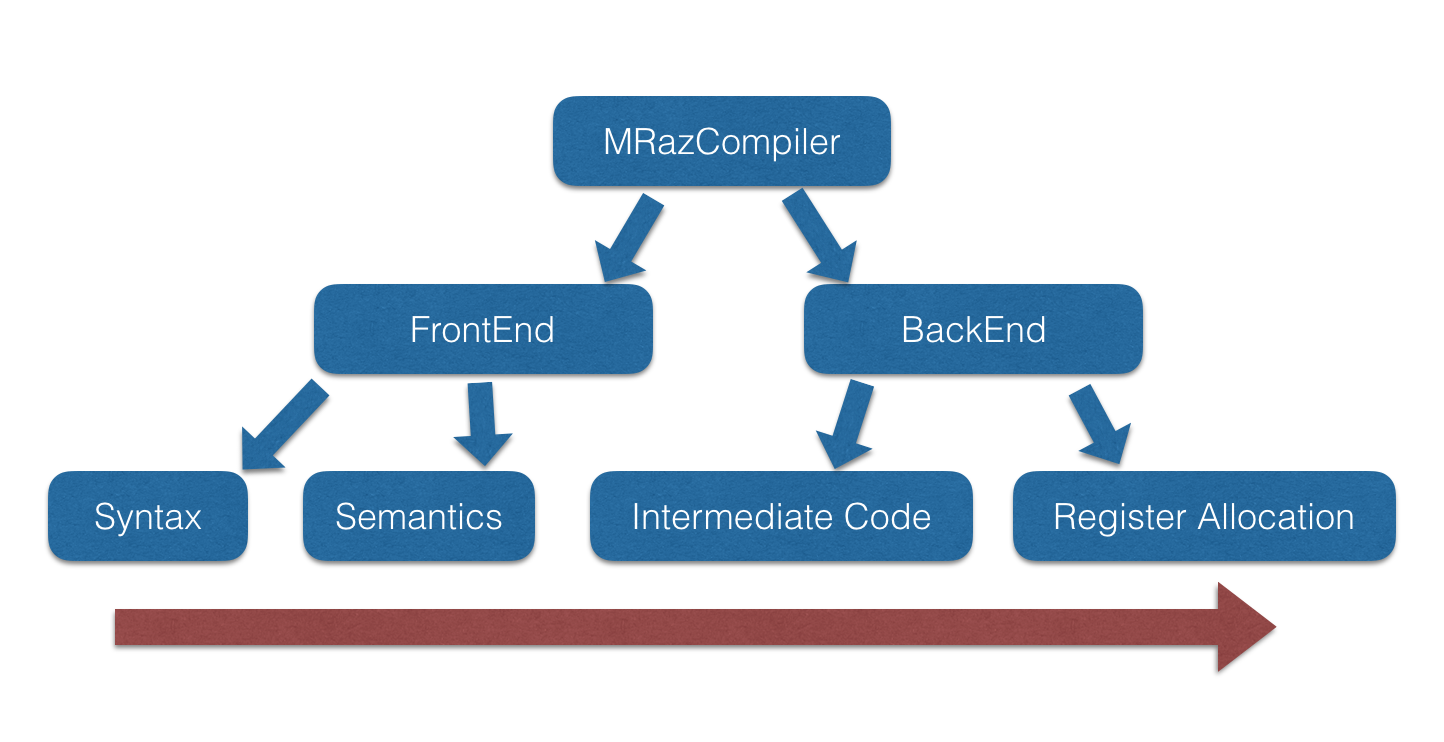
\includegraphics[width = \textwidth]{structure_1}
	\end{figure}
\end{frame}

\subsection{Features of My Compiler}
\begin{frame}
	\begin{itemize}
		\item clear thinking
		\item concise front end \& not too complicated back end
		\item good performance without re-run optimization
		\item ummm...actually it doesn't have any.
	\end{itemize}
\end{frame}

\section{Front-end Design}
\subsection{Syntax}
\begin{frame}
	\begin{figure}
		\centering
		
\includegraphics[width = \textwidth]{antlr}
	\end{figure}
	Rz.g4 $\Rightarrow$
	\[\begin{cases}
		\text{RzLexer: recognize and convert program into token stream} \\
		\text{RzParser: generate a parse tree (concrete syntax tree) }
	\end{cases}\]
\end{frame}

\subsection{Semantic}
\begin{frame}
	\begin{itemize}
		\item using RzBaseVisitor to travel on CST
		\item using SymbolTable to record identifier
		\item using TypeAnalyser to extract the \textbf{result type} and \textbf{identifier type} of expression
		\item the whole semantic check contains three rounds
	\end{itemize}
\end{frame}

\begin{frame}
	\begin{figure}
		\centering
		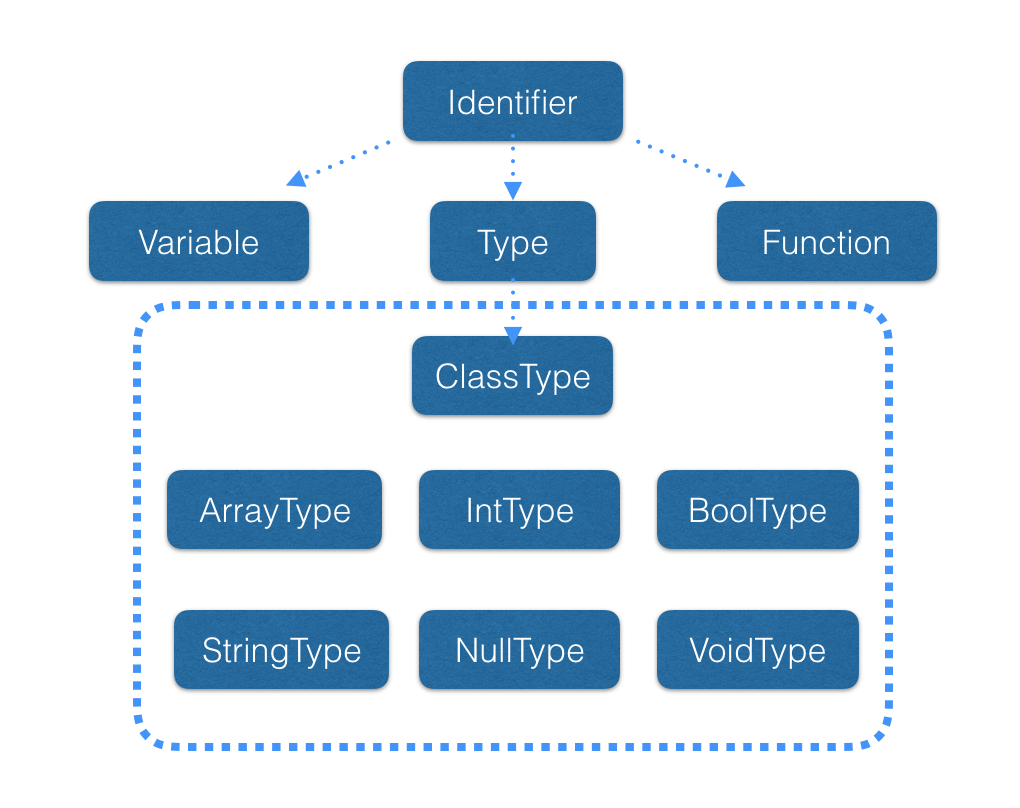
\includegraphics[width = 0.95\textwidth]{inheritance_1}
	\end{figure}
\end{frame}

\begin{frame}
	\begin{figure}
		\centering
		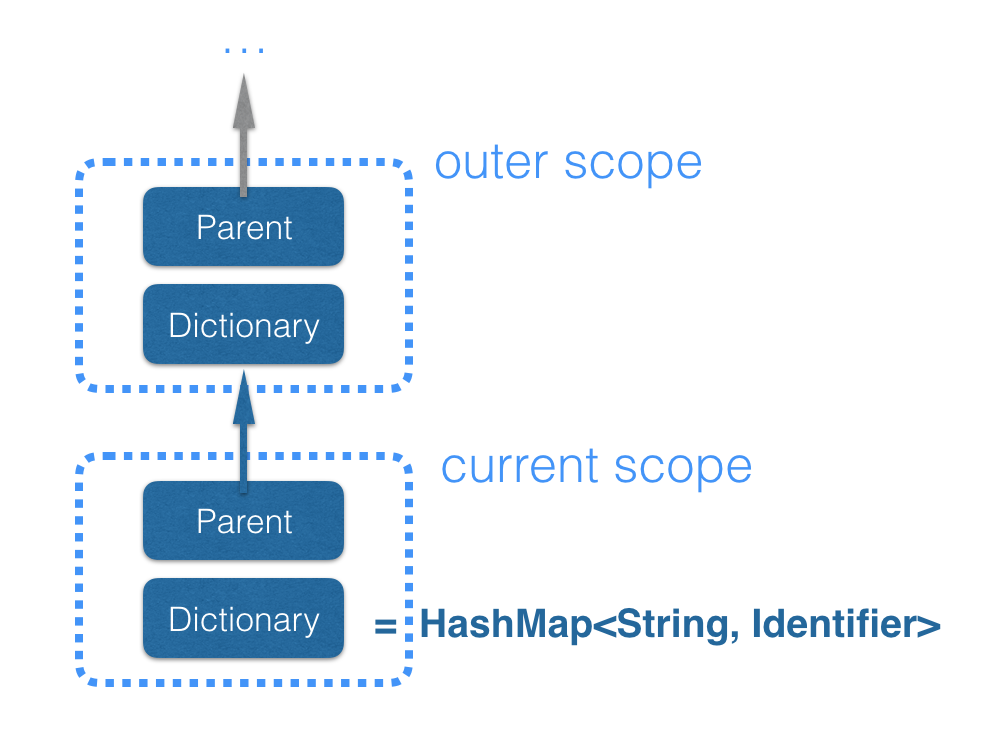
\includegraphics[width = 0.9\textwidth]{symboltable}
	\end{figure}
\end{frame}

\begin{frame} \frametitle{Type Analyzer}
	\begin{itemize}
		\item Downcast Pattern
		\item Result type: type of return values or variables
		\item Identifier type: a variable, a function or a resulted type of expression.
		\item type checking for expressions
	\end{itemize}
\end{frame}

\begin{frame} \frametitle{3 Rounds for Semantic Check}
	\begin{itemize}
		\item Round 1: GetClass
			\begin{itemize}
				\item add class name and set build-in functions to symbol table.	
			\end{itemize}
		\item Round 2: GetFuncAndClassMem
			\begin{itemize}
				\item get parameter list for each function
				\item get members for each class
				\item add functions and re-add class name to symbol table
			\end{itemize}
		\item Round 3: SemanticCheck
			\begin{itemize}
				\item check the program whether have a "main" function
				\item check the variable declaration and \textbf{update the symbol table}
				\item refresh the outer symbol table of the function
				\item link or recover the symbol table when enter or exit scope
				\item check the selection and iteration statement
				\item check the continue, break and return statement
			\end{itemize}
	\end{itemize}
\end{frame}

\subsection{Pretty Pirnt}
\begin{frame}\frametitle{Pretty Print}
	\begin{itemize}
		\item \textit{frontendText( parser, program, false, \underline{true} );}
	\end{itemize} 
	\begin{figure}
		\centering
		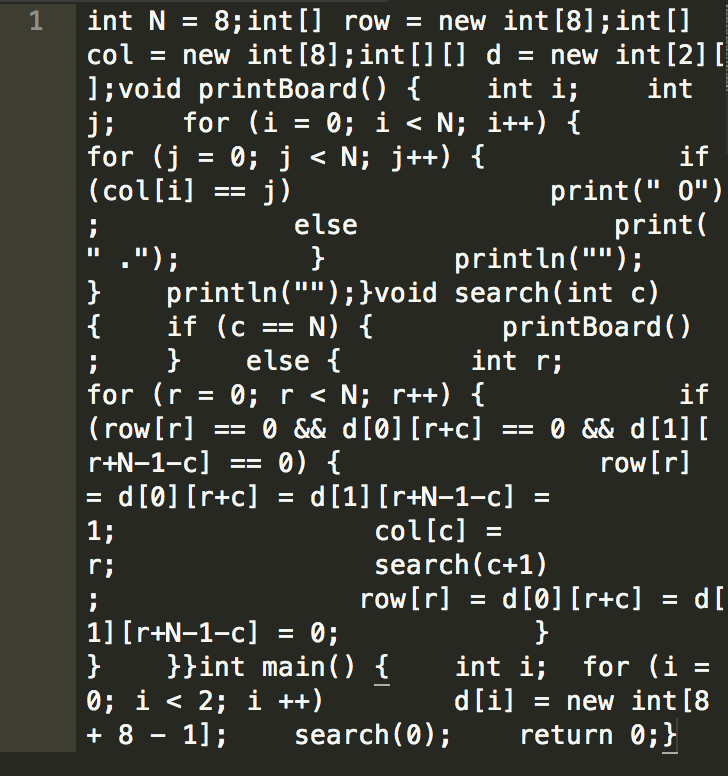
\includegraphics[width = 0.499\textwidth]{pp_1}
		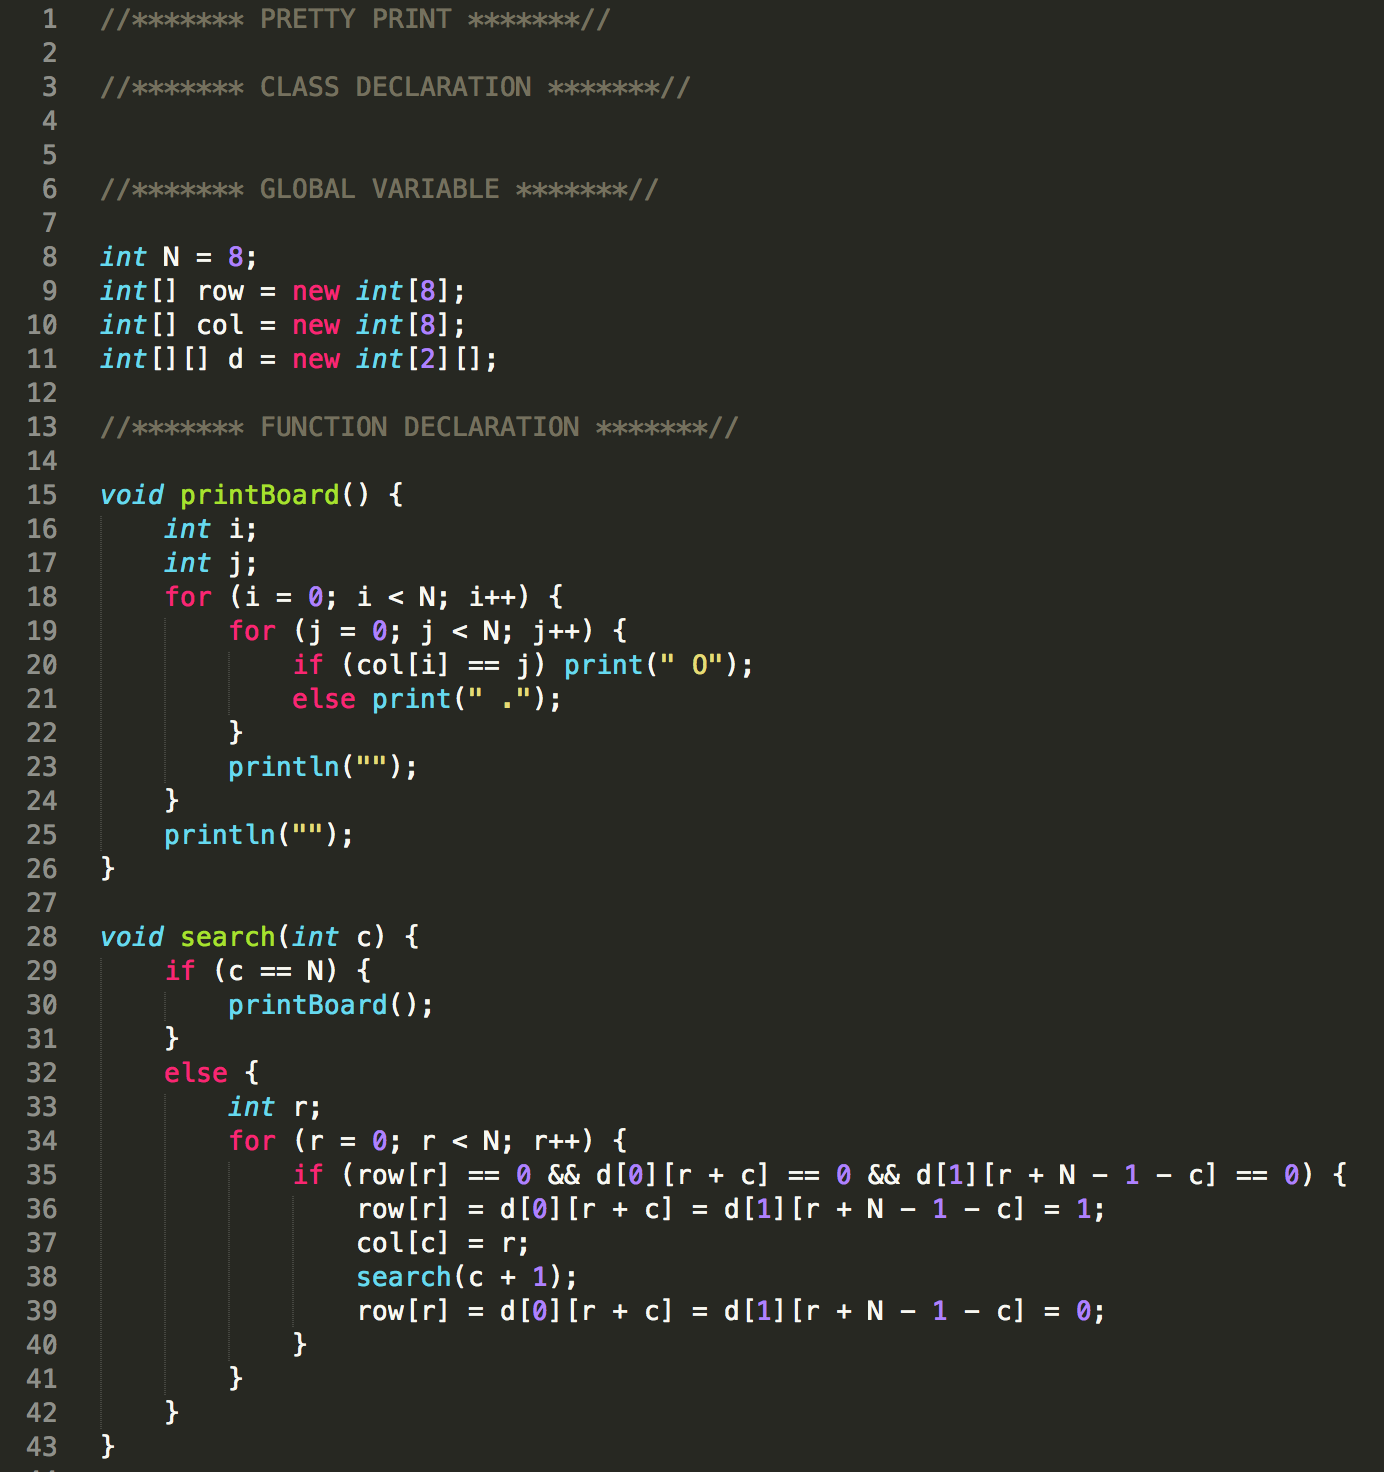
\includegraphics[width = 0.5\textwidth]{pp_2}
	\end{figure}
\end{frame}

\section{Back-end Design}
\subsection{Intermediate Representations}
\begin{frame}
	\begin{figure}
		\centering
		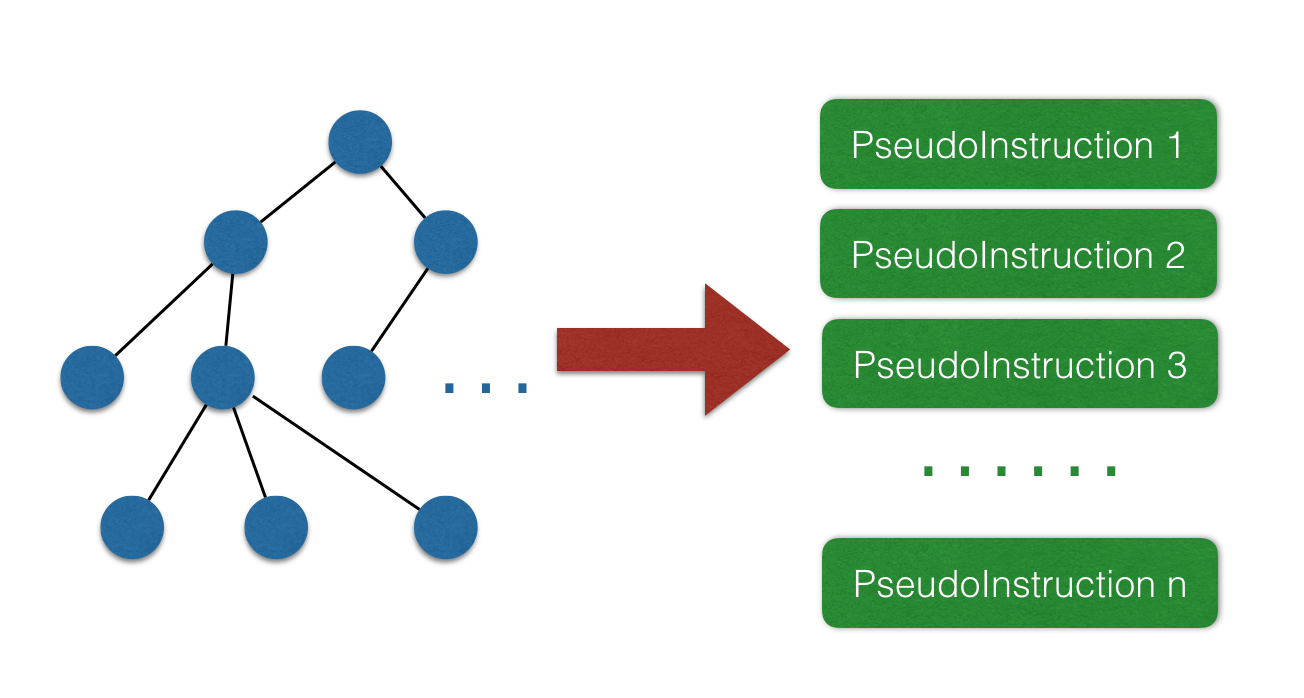
\includegraphics[width = \textwidth]{ir_0}
	\end{figure}
\end{frame}

\begin{frame}
	\begin{figure}
		\centering
		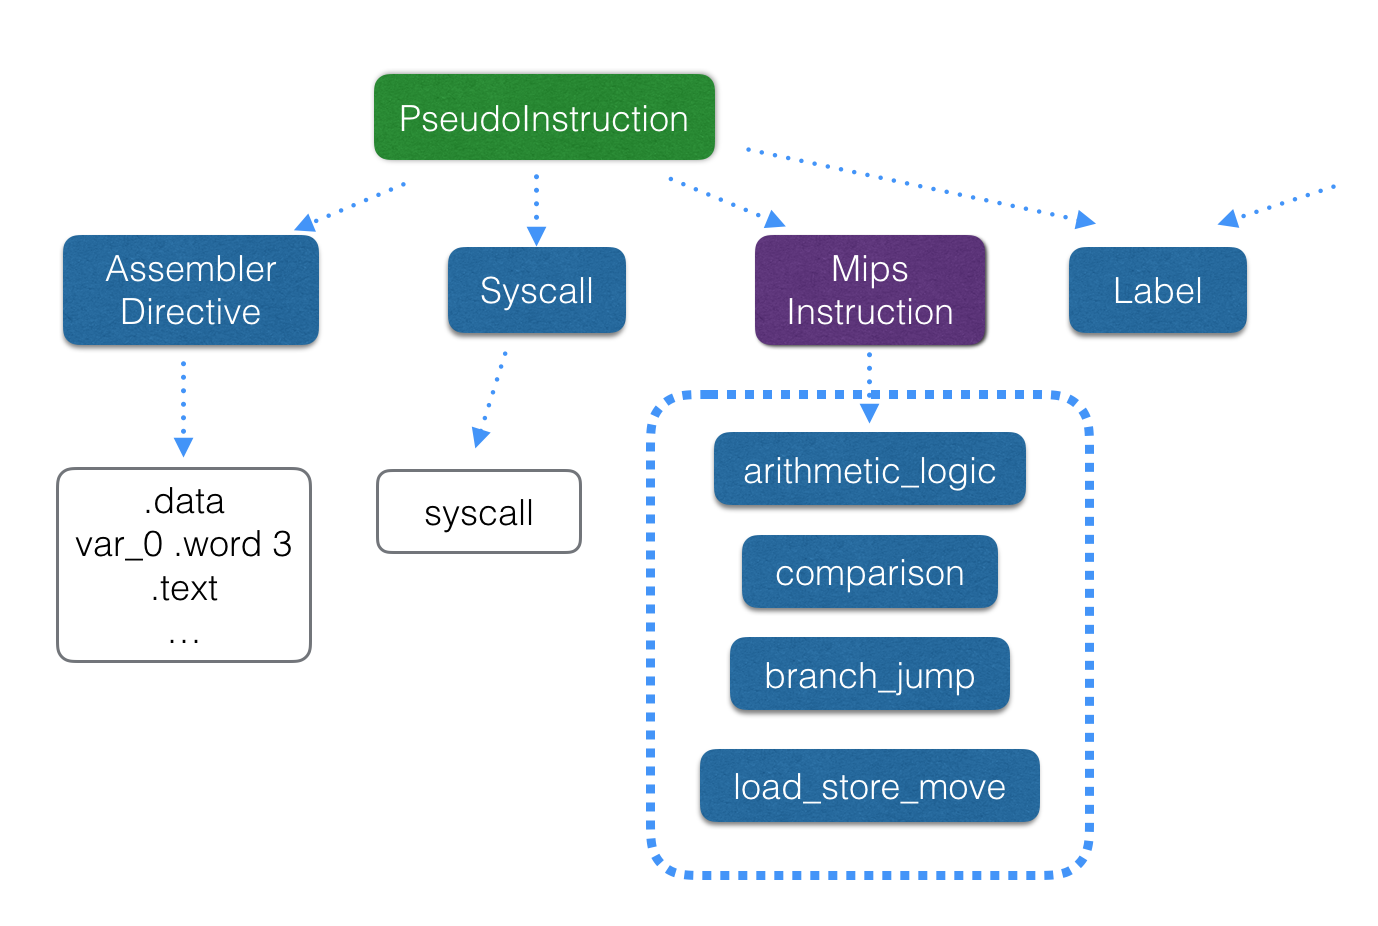
\includegraphics[width = \textwidth]{ir_1}
	\end{figure}
\end{frame}

\begin{frame}
	\begin{figure}
		\centering
		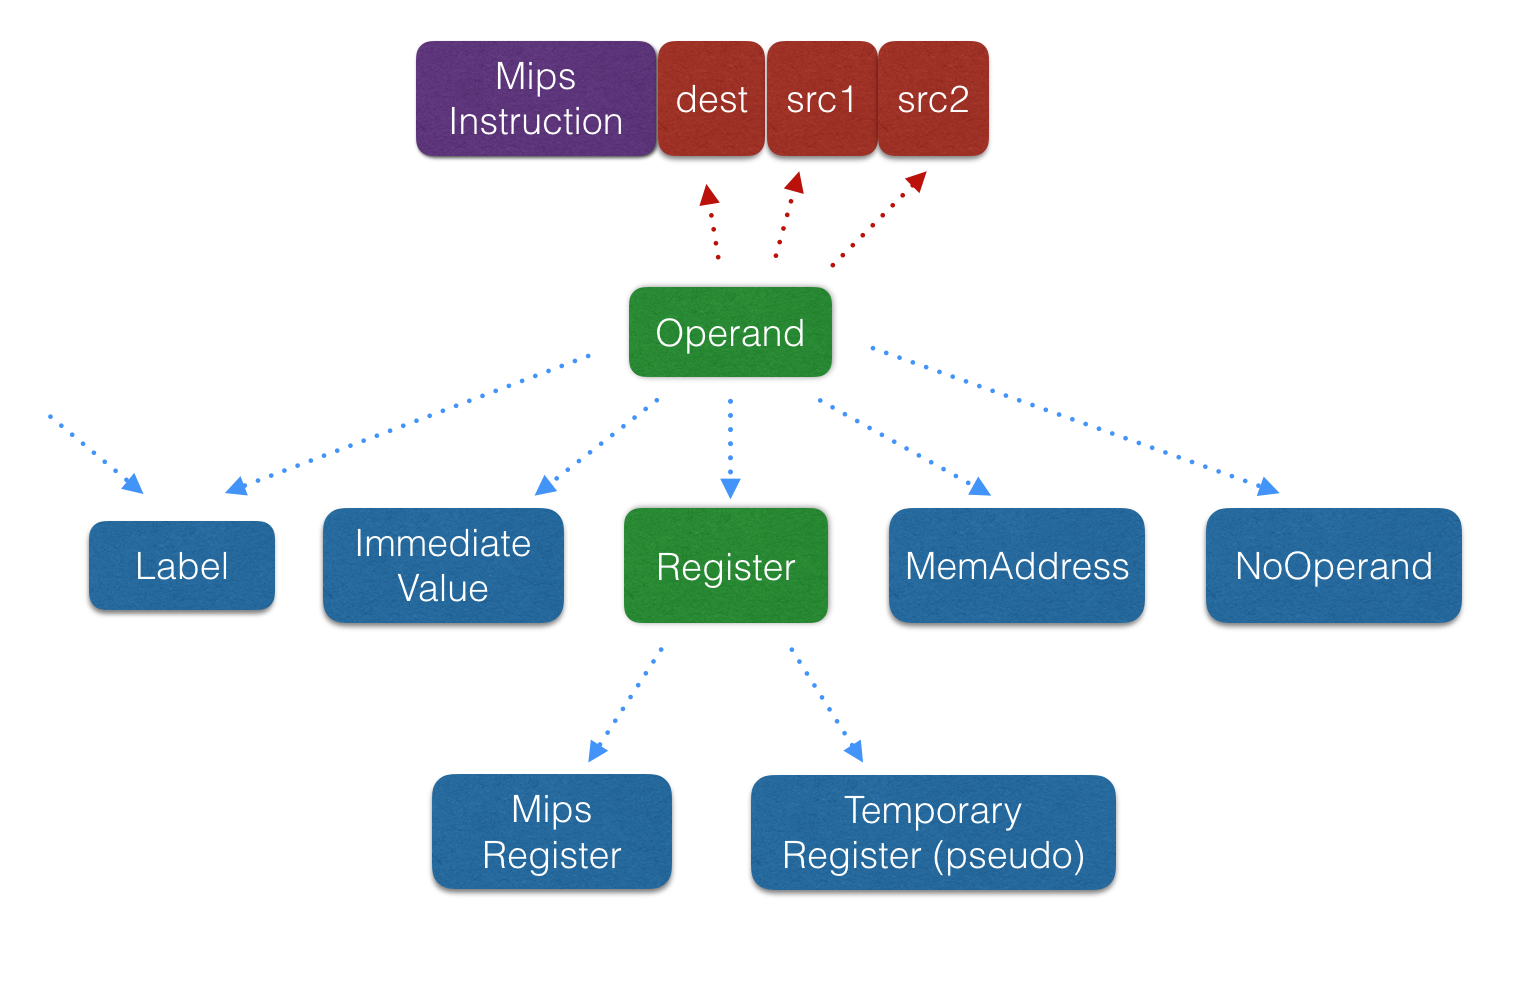
\includegraphics[width = \textwidth]{ir_2}
	\end{figure}
\end{frame}

\begin{frame}\frametitle{Three Minor Things}
	\begin{itemize}
		\item StringConstGetter
			\begin{itemize}
				\item extract string constants \& add them to data section
				\item make a dictionary for looking up corresponding label of each string const
			\end{itemize}
		\item PreIntermediateCodeTranslator
			\begin{itemize}
				\item extract global constants \& initialize them in data section
				\item if the initialization is complicated, then move those instructions to the beginning of main function.
			\end{itemize}
		\item SeparateIntermediateCodeTranslator
			\begin{itemize}
				\item translate each function to list of pseudo-instructions
			\end{itemize}
	\end{itemize}
\end{frame}

\begin{frame}\frametitle{IntermediateCodeTranslator}
	\begin{itemize}
		\item Visitor Pattern
		\item TemporaryRegisterGenerator produces unique temporary register (pseudo) for every variable and intermediate result
		\item synchronize the value of global variables, class type variables and array type variables between register and memory
		\item constant folding: i = 320 * 200 * 32;
		\item calculate the minimal offset for \$sp
	\end{itemize}
\end{frame}

\subsection{Calling Convention}
\begin{frame}
	\begin{figure}
		\centering
		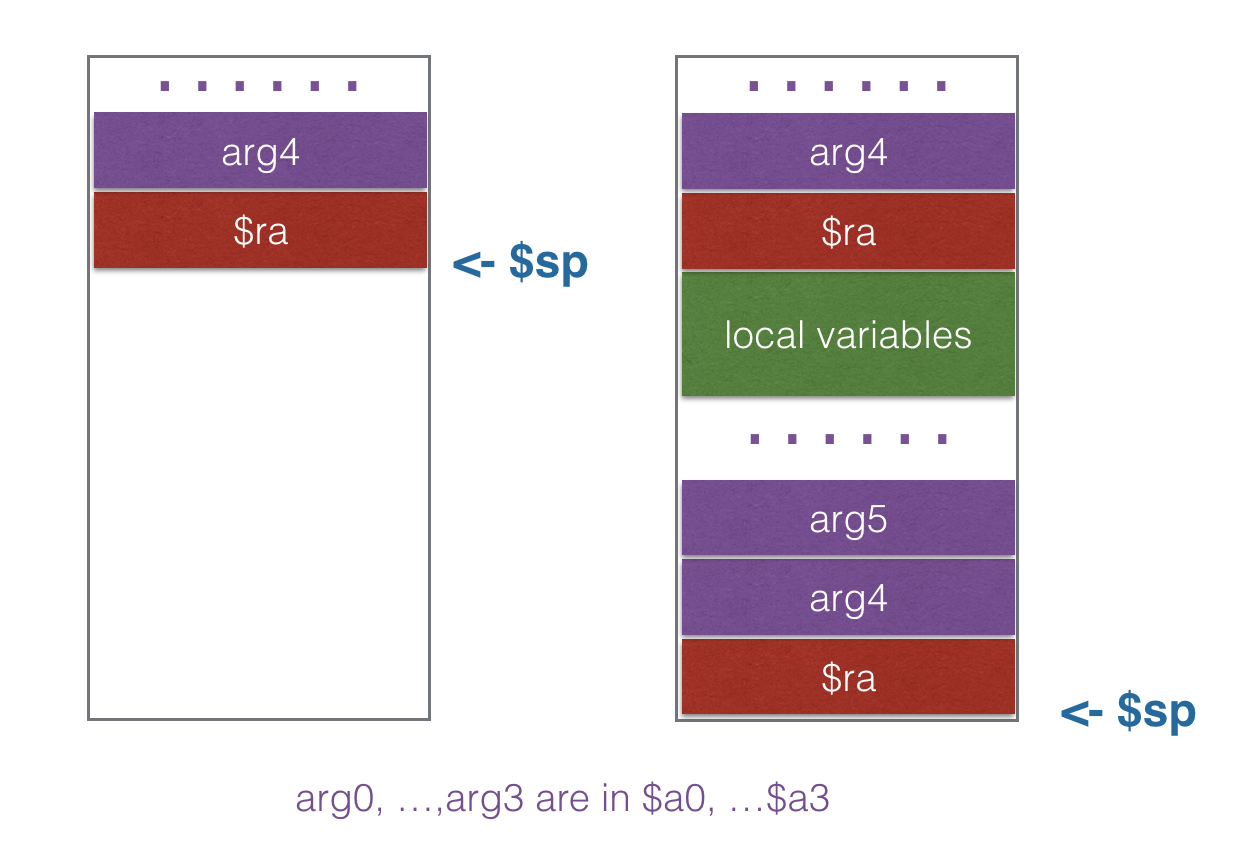
\includegraphics[width = \textwidth]{cc_1}
	\end{figure}
\end{frame}

\subsection{Register Allocation}
\begin{frame}
	\begin{figure}
		\centering
		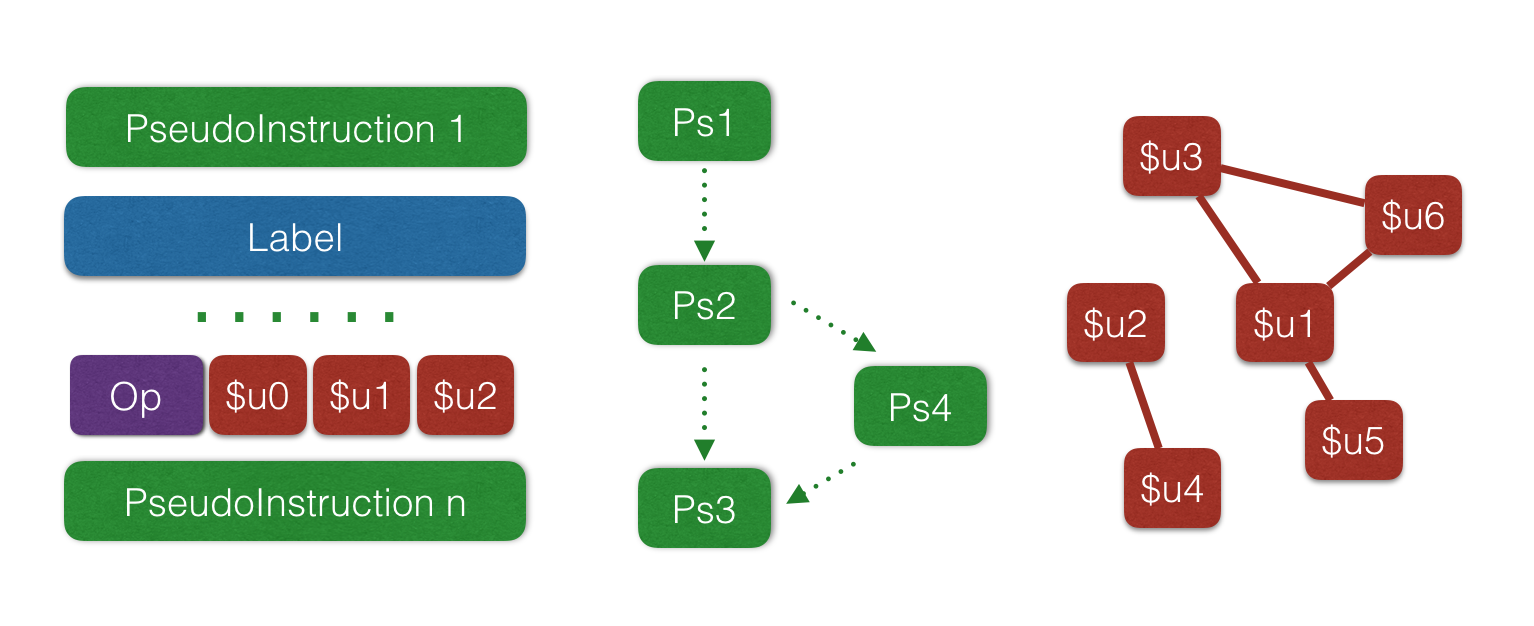
\includegraphics[width = \textwidth]{ra_1}
	\end{figure}
\end{frame}

\begin{frame}
	\begin{figure}
		\centering
		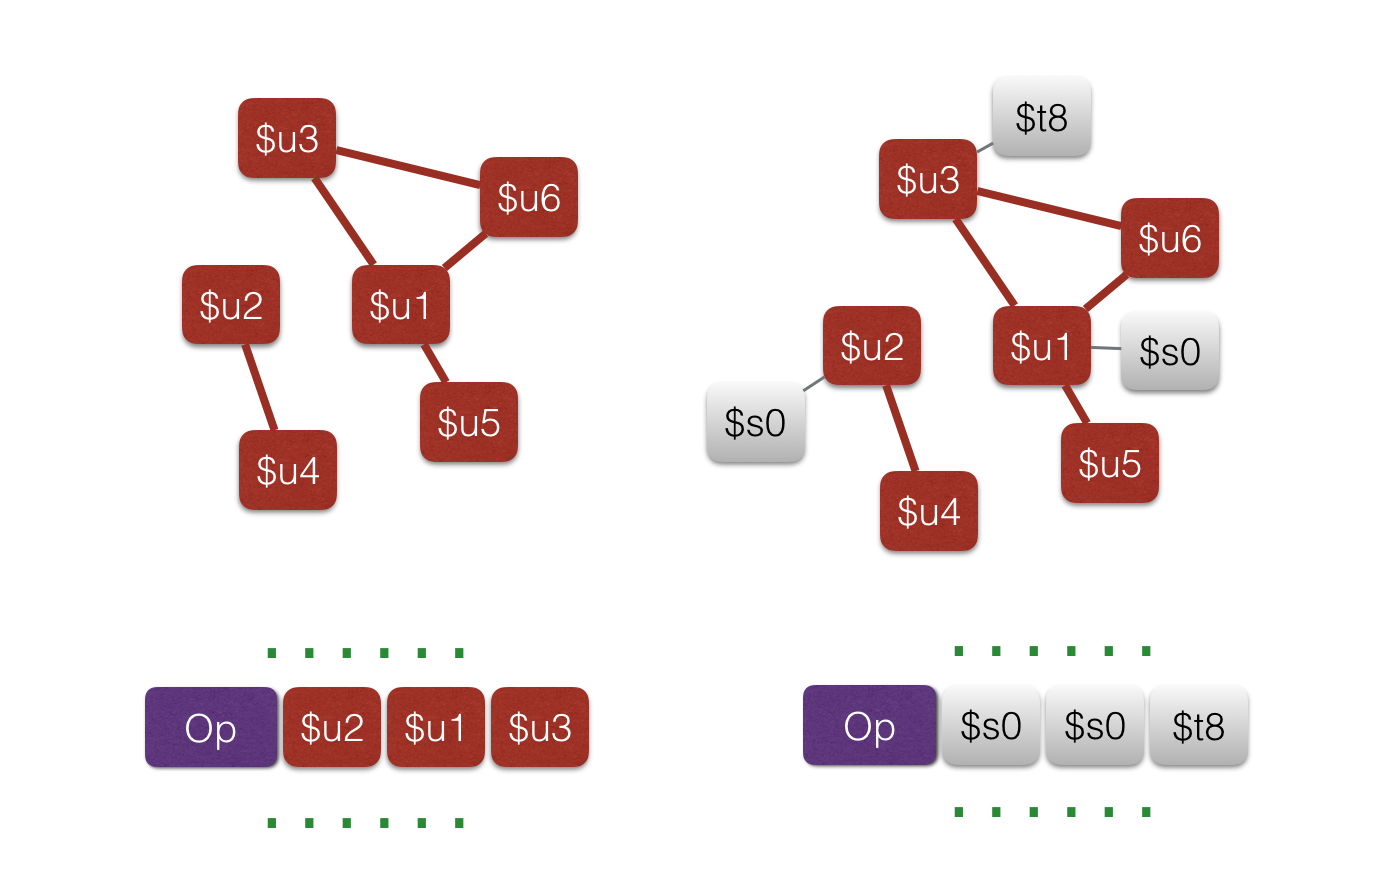
\includegraphics[width = \textwidth]{ra_2}
	\end{figure}
\end{frame}

\begin{frame}\frametitle{Control Flow Graph}
	\begin{itemize}
		\item each node represents a non-label pseudo-instruction
			\begin{itemize}
				\item DefinedRegisterGetter, UsedRegisterGetter
			\end{itemize}
		\item backward visit the pseudo-instruction list
		\item make a dictionary for label and its next non-label instruction
		\item make a CFG node when meeting a non-label instruction
		\item pull an edge from current node to previous node
		\item adapt branch and jump instruction with dictionary
	\end{itemize}
\end{frame}

\begin{frame}\frametitle{Interference Graph}
	\begin{itemize}
		\item calculate liveIn and liveOut for each node
			\begin{itemize}
				\item $\text{liveIn} = Uses \cup (\text{liveOut} - Defs)$
				\item $\text{liveOut} = \bigcup_{succ}\text{liveIn}$
			\end{itemize}
		\item do iteration until they are unchanged
		\item \textbf{tag the instruction if its def temp reg in not in liveOut}
		\item connect two register if they are in the same liveOut.
	\end{itemize}
\end{frame}

\begin{frame}\frametitle{FrameManager}
	\begin{itemize}
		\item Cast to Memory
			\begin{itemize}
				\item allocate a memory address to real register
				\item update the size of stack frame
			\end{itemize}
		\item Back from Memory
			\begin{itemize}
				\item re-load the data from memory to history register
			\end{itemize}
		\item record register \& count minimal offset
	\end{itemize}
\end{frame}

\begin{frame}
	Linear scan the untagged pseudo-instruction in list, for each operand:
	\begin{itemize}
		\item if the temporary register has no history
			\begin{itemize}
				\item available = \{\$t0,...,\$t9,\$s0,...\$s7\} - $\bigcup_{\text{adjacent}}$ realRegister
				\item if available $ = \emptyset$, cast one adjacent temp reg to memory, set real register as this one's
				\item else set real register as some one in available
			\end{itemize}
		\item if the temporary register has a history register
			\begin{itemize}
				\item if the history register $\notin \bigcup_{\text{adjacent}}$ realRegister, then set the real register as the history
				\item else cast the adjacent one to memory, and set the real register as the history
			\end{itemize}
		\item real register, immediate value and label, just keep them
	\end{itemize}
\end{frame}

\begin{frame}
	\begin{itemize}
		\item When meeting "jal" instruction, cast all temporary register registers in its liveIn to memory before calling, and pull them back after calling. 
		\item Correct \$sp movement and clean up history every time after register allocation.
		\item use InstructionPrinter to print the mips assemblers.
	\end{itemize}
\end{frame}

\begin{frame}\frametitle{Special Case}
	\begin{itemize}
		\item Spill2: CiscRegisterAllocator
			\begin{itemize}
				\item Too many CFGNodes \& Too dense IG
				\item Why not use only three registers, then load, load, store.
			\end{itemize}
	\end{itemize}	
\end{frame}

\section{Performance}
\subsection{Summary}
\begin{frame}
	\begin{figure}
		\centering
		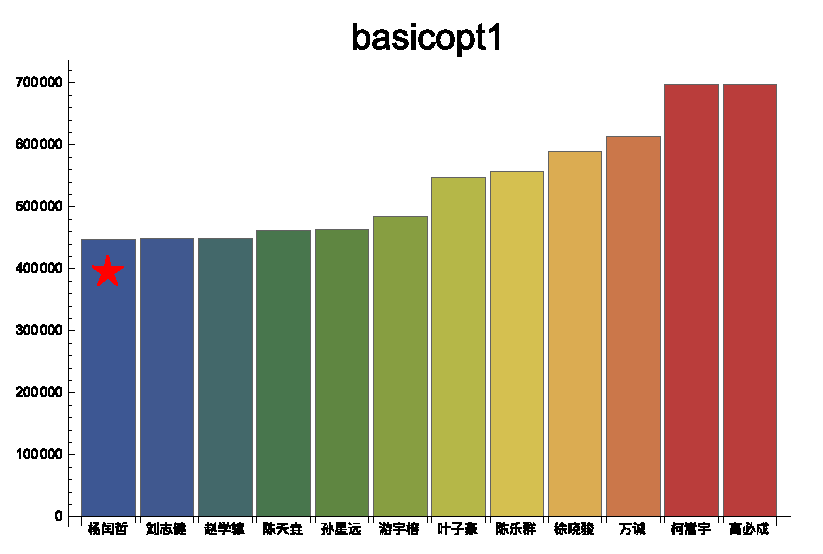
\includegraphics[width = \textwidth]{cr_2}
	\end{figure}
\end{frame}

\begin{frame}
	\begin{figure}
		\centering
		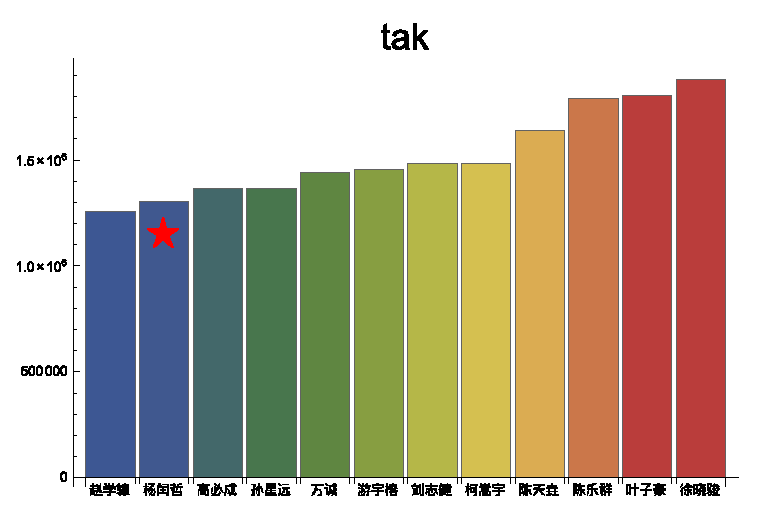
\includegraphics[width = \textwidth]{cr_9}
	\end{figure}
\end{frame}

\begin{frame}
	\begin{figure}
		\centering
		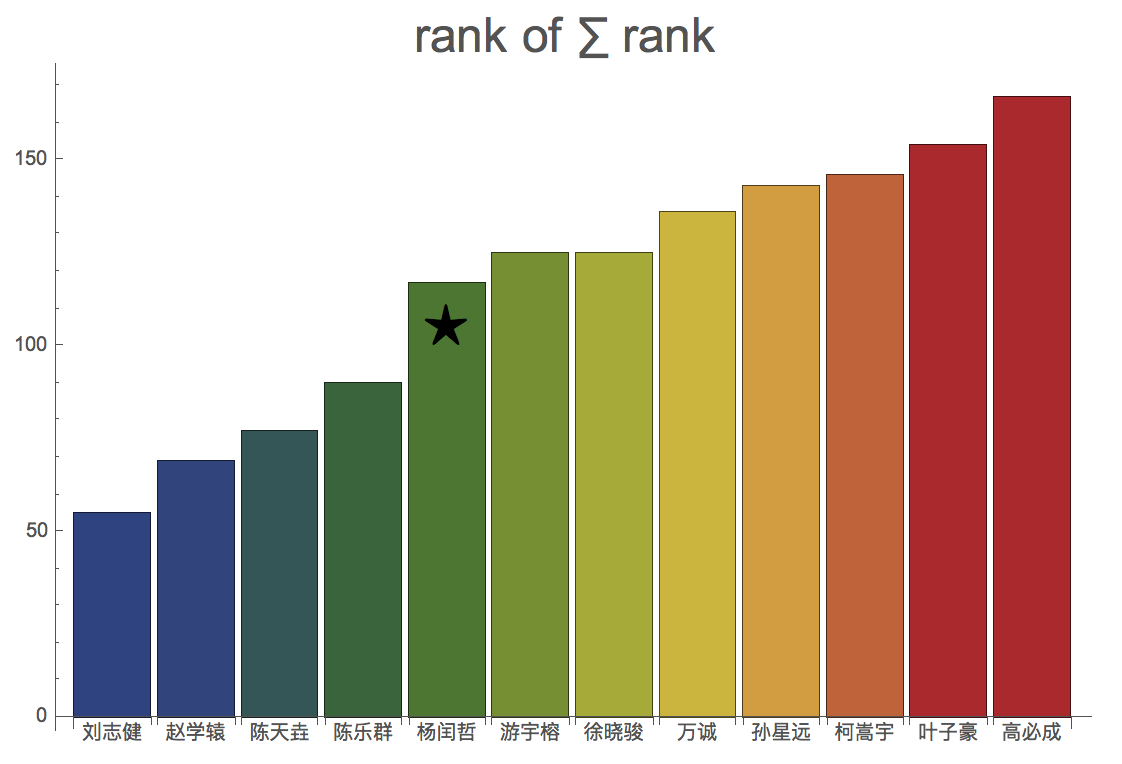
\includegraphics[width = \textwidth]{rankofrank.png}
	\end{figure}
\end{frame}

\subsection{Potential Optimization}
\begin{frame}
	\begin{itemize}
		\item More precise def-use relationships
			\begin{itemize}
				\item constant propagation
				\item dead code elimination
			\end{itemize}
		\item Make short functions inline \& opt print(toString(a) + " ")
		\item Loop optimizations
			\begin{itemize}
				\item loop unrolling
				\item loop fusion
				\item software pipelining
			\end{itemize}
		\item Delete redundant memory operations before and after a function call
	\end{itemize}
\end{frame}

\section{Acknowledgement}
\begin{frame}
	\begin{figure}
		\centering
		
\includegraphics[width = \textwidth]{end_1}
	\end{figure}
\end{frame}

\end{document}
